	
\subsubsection{21.10.14}

\begin{enumerate}
	\item Время начала и окончания собрания:\newline
	17:00 - 19:00
	\item Цели собрания:\newline
	\begin{enumerate}
	  \item Еще раз обдумать стратегию автономного и финального периодов и в случае необходимости внести поправки.\newline
	  
	  \item Закончить установку ребер жесткости на направляющие подъемник.\newline
	  
	  \item Установить нижние ограничители для мебельных реек.\newline
	  
    \end{enumerate}
    
	\item Проделанная работа:\newline
	\begin{enumerate}
	  \item Ребра жесткости установлены на подъемник.\newline
      
      \item Устранена проблема проваливания реек путем укрепления стандартных ограничителей термоклеем.\newline
      
      \begin{figure}[H]
      	\begin{minipage}[h]{0.31\linewidth}
      		\center{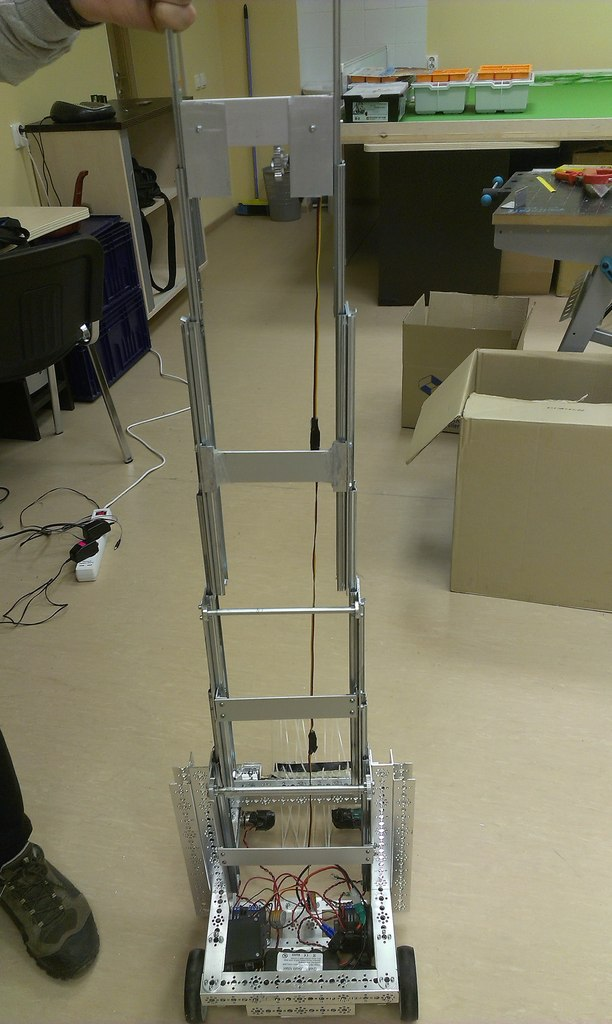
\includegraphics[height=0.8\measurepage]{days/images/PKDWalSyXpU}}  
      	\end{minipage}
      	\hfill
      	\begin{minipage}[h]{0.31\linewidth}
      		\center{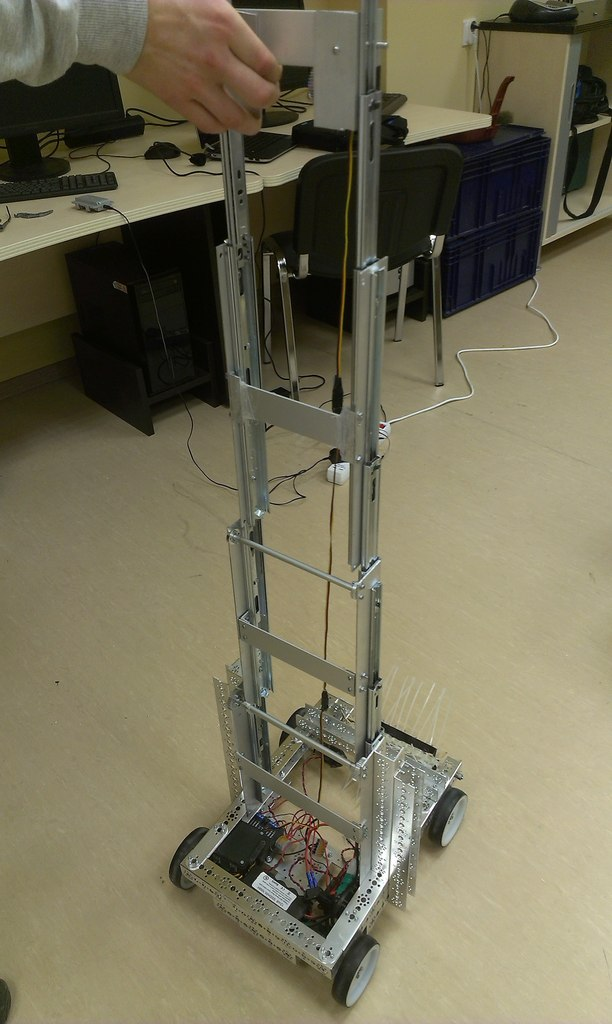
\includegraphics[height=0.8\measurepage]{days/images/BwFbxLqFx8A}} 
      	\end{minipage}
      	\hfill
      	\begin{minipage}[h]{0.31\linewidth}
      		\center{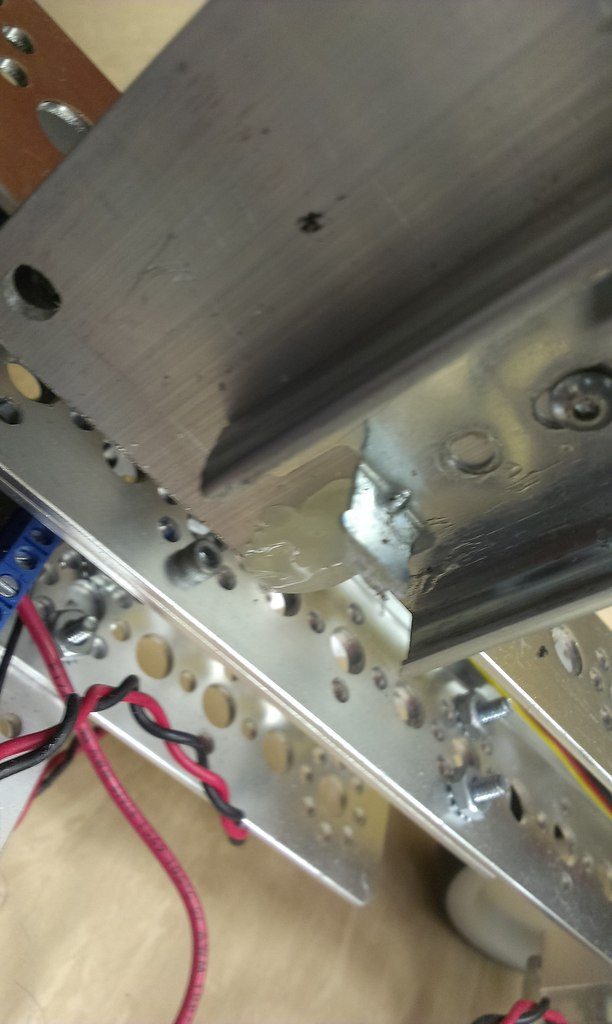
\includegraphics[height=0.8\measurepage]{days/images/Um_IaFnAhTI}}
      	\end{minipage}
      	\vfill
      	\begin{minipage}[h]{0.665\linewidth}
      		\caption{Ребра жесткости установлены на робота}  
      	\end{minipage}
      	\hfill
      	\begin{minipage}[h]{0.31\linewidth}
      		\caption{Ограничители хода мебельных реек укреплены термоклеем}  
      	\end{minipage}
      \end{figure}
      
      \item Была еще раз обдумана стртегия автономного и финального периодов. Поправок внесено не было.\newline
      
      \item В конце собрания произошла поломка одной из мебельных реек (выскочила верхняя часть). Это необходимо исправить.\newline
      
      \begin{figure}[H]
      	\begin{minipage}[h]{0.2\linewidth}
      		\center   
      	\end{minipage}
      	\begin{minipage}[h]{0.6\linewidth}
      		\center{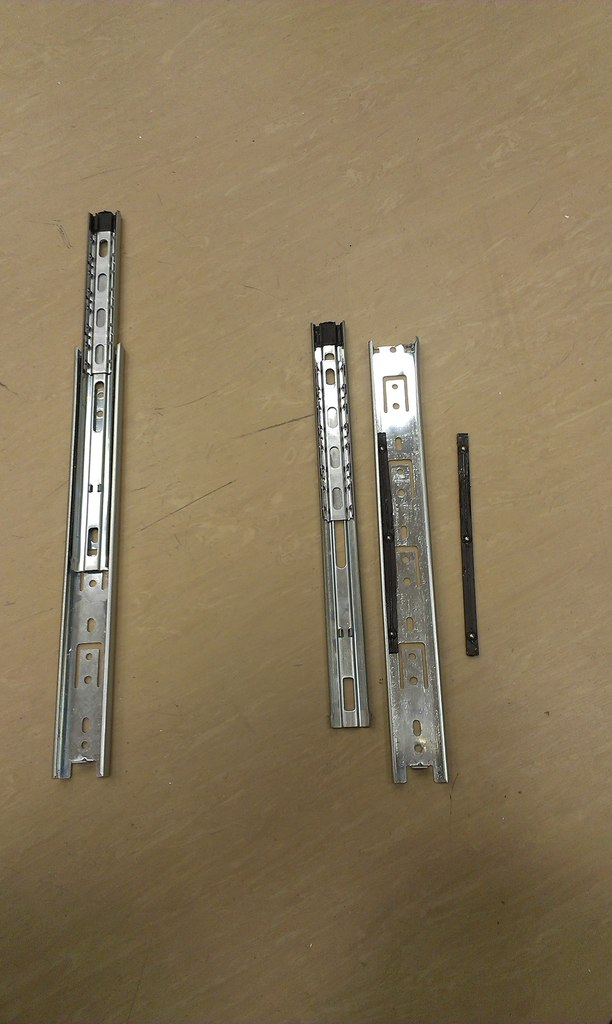
\includegraphics[height=0.95\measurepage]{days/images/6nL5z3edN6A}}
      		\caption{Поломанная мебельная рейка (справа)}
      	\end{minipage}
      \end{figure}
      
    \end{enumerate}
    
	\item Итоги собрания: \newline
	\begin{enumerate}
	  \item Все ребра жесткости установлены.\newline
	  
      \item Установлены нижние ограничители мебельных реек.\newline
      
    \end{enumerate}
    
	\item Задачи для последующих собраний:\newline
	\begin{enumerate}
	  \item Исправить поломку рейки, понять в чем ее причина и как этого избежать в дальнейшем.\newline
	  
    \end{enumerate}     
\end{enumerate}

\fillpage
